\pagestyle{fancy}
\fancyhead[l]{\autorUO}
\fancyfoot[l]{\asignaturaAbbr}
\fancyfoot[r]{\fecha}

\section{\rowmajor\ vs \colmajor} \label{sec:3}
En esta sección se comparan los dos métodos de recorrido de matrices, \rowmajor\ y \colmajor, en cuanto a su rendimiento en el producto matricial.
Para ello, se ha realizado dicha operación para los siguientes tamaños de matrices: 
$\{2,\ 4,\ 8,\ 16,\ 32,\ 64,\ 128,\ 256,\ 398,\ 512,\ 636,\ 774,\ 892,\ 1024,\ 1152,\ 1280,\ 1408,\ 1536\}$. Cada producto se ha realizado un total 
de 32 veces y se ha medido el tiempo medio de ejecución. Los resultados obtenidos se presentan en la \autoref{fig:1}.

\begin{figure}[h]
    \centering
    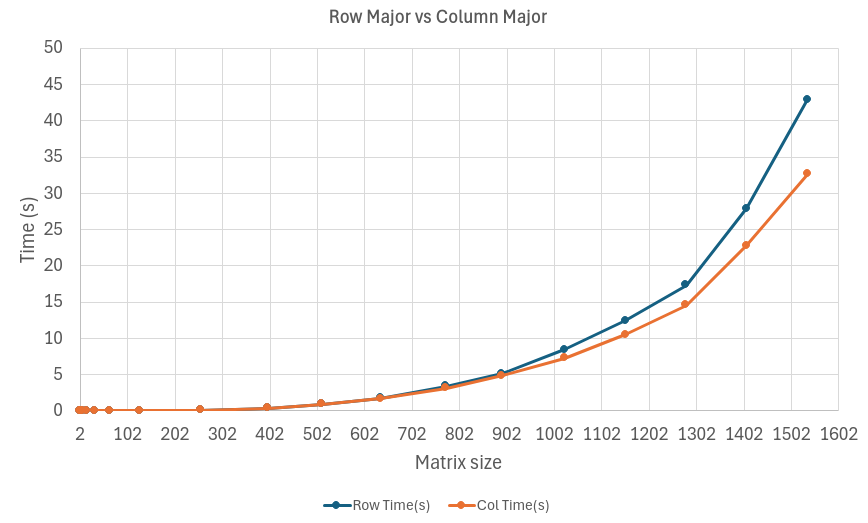
\includegraphics[width=0.5\textwidth]{img/1.png}
    \caption{Comparación de tiempos de ejecución para \rowmajor\ y \colmajor}
    \label{fig:1}
\end{figure}

Sorprendentemente, el recorrido por columnas es más rápido que el recorrido por filas. Esta diferencia comienza a ser notable 
a partir de un tamaño de matriz relativamente grande, aproximadamente de $1024 \times 1024$.
Dicha diferencia crece a medida que aumenta el tamaño de la matriz, alcanzando unos $10s$ de diferencia en el mayor tamaño de matriz 
probado ($1536 \times 1536$).
Para representar la diferencia de rendimiento entre ambos métodos, se ha calculado la aceleración de \rowmajor\ respecto a \colmajor\ para cada tamaño de matriz.
Dicha aceleración se ha graficado en la \autoref{fig:2}.

\begin{figure}[h]
    \centering
    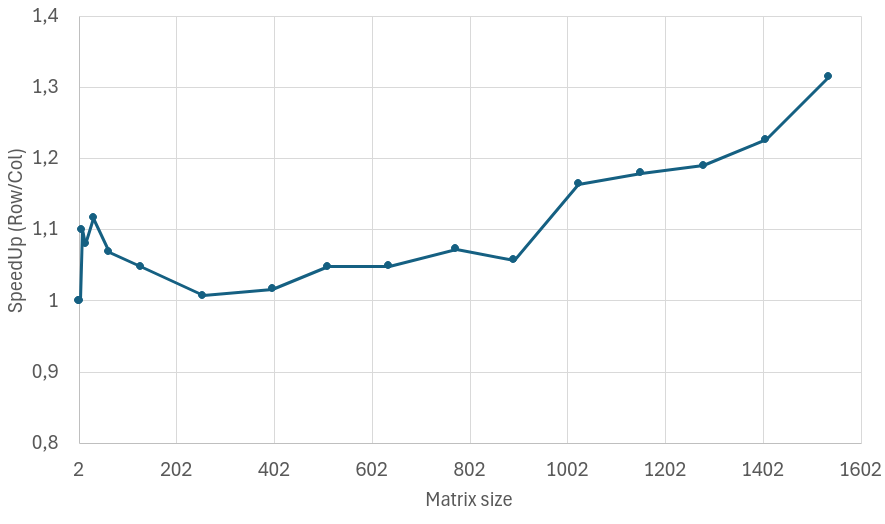
\includegraphics[width=0.5\textwidth]{img/2.png}
    \caption{Aceleración de \rowmajor\ respecto a \colmajor}
    \label{fig:2}
\end{figure}

Como puede observarse, \colmajor\ es más rápido que \rowmajor\ para todos los tamaños de matriz probados, siendo notablemente 
mejor conforme aumenta el tamaño de la matriz. Esto se ve reflejado en la tendencia creciente de la aceleración graficada.